\chapter{Metodología}
\label{cap:metodologia}
En este capítulo se explicará todo lo relacionado con la metodología utilizada en este Trabajo Fin de Grado. Con el objetivo de encontrar una solución sostenible, flexible en términos de negocio y que sea capaz de amoldarse a las especificaciones y criterios del proyecto.\\\\

En primer lugar, se realizará una introducción a los equipos utilizados en el proyecto tanto a nivel software como hardware. Se detallarán las especificaciones técnicas y características de los equipos, así como su motivación para ser usados en este proyecto. De la misma manera se explicará el funcionamiento del software de configuración disponible en los equipos.\\\\

En segundo lugar, se realizarán pruebas a nivel de laboratorio utilizando configuraciones similares a las utilizadas en el marco del proyecto Napo. Siguiendo un escenario base de laboratorio, se analizará el rendimiento de los equipos a nivel de red, utilizando para ello herramientas cuya funcionalidad será la inyección de tráfico simulado. De forma paralela se utilizará la solución propuesta en el capítulo \ref{cap:marco_teorico} para realizar la gestión y monitorización de redes sobre el escenario red disponible en laboratorio.

\section{Equipos propuestos}
Con el objeto de seleccionar aquellos equipos que mejor rendimiento y prestaciones ofrezcan al proyecto, se ha establecido una comparativa y estudio entre diferentes propuestas. Dichas propuestas no sólo deben adaptarse y cumplir a los requerimientos técnicos del proyecto, si no que también deben mostrar un rendimiento adecuado al coste establecido por el proyecto.\\\\

Para ello, y con la ayuda de la PUCP se ha establecido un protocolo de pruebas que nos mostrará el rendimiento de los equipos sobre pruebas realizadas en campo. Dichas pruebas determinarán qué equipos son los finalmente seleccionados como solución del proyecto. A continuación, se procede a detallar cada uno de los equipos involucrados en este estudio y la comparativa entre ellos.

\subsection{Equipos Ubiquiti: AirFiber AF-5X}
Los equipos AirFiber son equipos pertenecientes a la empresa estadounidense Ubiquiti Networks \cite{Ubiquiti}. Esta empresa se dedica principalmente al desarrollo y comercialización de dispositivos para redes inalámbricas, ya sean de larga o corta distancia. Los equipos desarrollados por la empresa se caracterizan por su alto rendimiento y su bajo coste. \\\\

Actualmente existe una gran variedad de dispositivos diseñados para redes inalámbricas, en nuestro caso utilizaremos el modelo AirFiber AF-5x, perteneciente a la familia AF de dispositivos radio. La pecularidad de este modelo es la utilización de la banda de 5 GHzs como frecuencia operacional, y no sólo eso, si no que además este modelo abarca todo el espectro radioeléctrico en el rango de 5 GHzs, tanto las bandas licenciadas como las que no lo son. Aparte de esto, estos equipos permiten ajustar el ancho de banda operacional, en el caso del modelo AF-5X de 10 a 50 MHzs, en intervalos de 10 MHzs otorgando mayor flexibilidad a la configuración de canales de subida y de bajada. Además de esto, los equipos permiten ajustar los canales de transmisión y recepción evitando así que existan interferencias en los canales seleccionados.

\subsubsection{Hardware}
Los dispositivos AF-5x están diseñados con una carcasa de silicona que recubre la placa empotrada que forma el equipo, tal y como se muestra en la figura \ref{af_5x}, el diseño sencillo de los equipos y sus conexiones salientes hacen de él un equipo muy versátil y flexible a la hora de ser integrado con otros componentes, como por ejemplo una antena o un sistema empotrado sobre una torre. Aparte de su flexibilidad a nivel físico, también ofrece gran versatilidad en su comportamiento, permitiendo así utilizar este equipo en diferentes roles según requiera la arquitectura diseñada, ya sea bien como estación base, o como un repetidor. De igual forma, su sistema está diseñado para ofrecer el máximo rendimiento de la transmisión mediante la reducción de señales interferentes y habilitando la posibilidad de utilizar constelaciones mayores para obtener un mayor \textit{trhoughput}.

\begin{figure}[H]
		\centering
		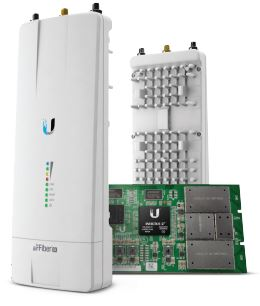
\includegraphics[width=5cm,height=5cm]{img/af_5x.JPG}
		\caption{Dispositivo AF-5X}
		\label{af_5x}
	\end{figure}
	
\subsubsection{Software}
Los equipos propietarios de la marca Ubiquiti utilizan un \textit{software} propietario que permite controlar y configurar los equipos. Aunque no esté en su versión final, el programa Ubiquiti Network Management System (UNMS) otorga al usuario un control absoluto sobre los dispositivos que conforman la red, y una serie de aplicaciones internas para obtener una correcta parametrización del rendimiento de los equipos. Tal y como se muestra en la figura \ref{unms} podemos ver como la pantalla principal del \textit{software} muestra diferentes tipos de configuración, paneles de interacción con el usuario, así como diferentes pestañas en las cuales se muestran datos a tiempo real del rendimiento de los equipos. 

\begin{figure}[H]
		\centering
		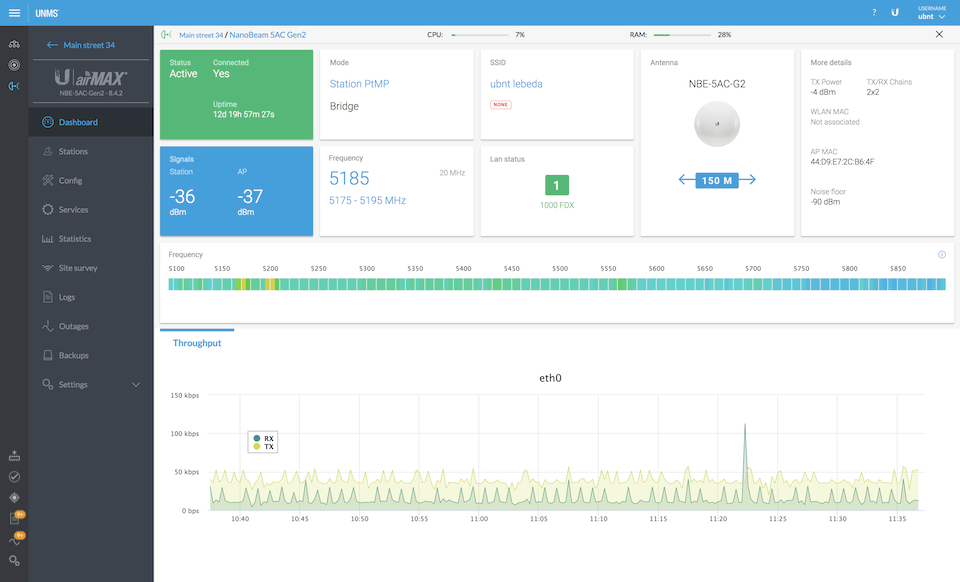
\includegraphics[width=0.5\textwidth]{img/unms.png}
		\caption{Pantalla principal UNMS}
		\label{unms}
	\end{figure}
	
Aparte de las funcionalidades antes comentadas, UNMS ofrece la posibilidad de obtener datos referentes al rendimiento de los equipos en lo que a parametrización de red respecta, es decir, todo lo relacionado con tráfico entrante y saliente de la red, niveles de recepción de señal, etc... Dichos parámetros pueden obtenerse utilizando una apicación interna que la propia herramienta tiene integrada consigo.

\subsection{Equipos VNL: RM-MAX}
Los equipos RM-MAX son dispositivos que pertenecen a las placas inalámbricas que fabrica y comercializada la empresa VNL \cite{VNL}. Fundada en 2004, VNL se dedica al desarrollo e implementación de equipos para infraestructuras de telecomunicaciones punto a punto. Aunque su principal enfoque estratégico sea en aplicaciones militares y civiles, actualmente existe una creciente demanda de uso de estos equipos en zonas rurales de países en vías de desarrollo, como por ejemplo India, Nepal o Indonesia.\\\\

Los equipos RM-MAX  utilizan OFDM como protocolo de acceso al medio, pero este procotocolo no es el nativo, es decir, es una variante propietaria de VNL que permite mantener las conexiones existentes de forma prolongada evitando caídas con la parte \textit{core} de la red. De igual forma, los equipos permiten un control absoluto sobre las transmisiones existentes en la red, consiguiendo así una reducción en costes importante evitando el uso de líneas cableadas. Otro factor a tener en cuenta, es que dichos equipos están fabricados y desarrollados bajo la metodología \textit{Plug and Play}, lo que quiere decir que su instalación y configuración se realiza forma rápida y sencilla.

\subsubsection{Hardware}
Los equipos RM-MAX escogidos como solución de este proyecto, son capaces de cubrir una distancia superior a los 100 Km incluyendo diferentes configuraciones según la frecuencia que deseemos usar. Tal y como se muestra en la figura \ref{rm_max}, la antena está integrada en una placa cuyo recubrimiento metálico hace que este equipo sea robusto frente a situaciones climatólogicas adversas. De igual forma dichos equipos están dotados de diferentes modos de funcionamiento, lo que permite mayor versatilidad a lo hora de configurar un tipo determinado de infraestructura, de igual forma estos equipos admiten diferentes modos de actuación, ya sea bien como estación base o como \textit{bridge}.

\begin{figure}[H]
		\centering
		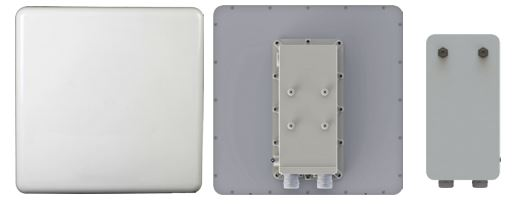
\includegraphics[width=0.5\textwidth]{img/rm_max.JPG}
		\caption{Dispositivo RM-MAX}
		\label{rm_max}
	\end{figure}
	
\subsubsection{Software}
Los equipos VNL utilizan como \textit{software} de gestión y configuración el \textit{Radio Modem Management}, dicho programa es propietario de VNL y muestra un aspecto similar al que se muestra en la figura \ref{vnl_rm}. Dicha aplicación permite configurar de manera sencilla los parámetros de red deseables en cuanto a configuración se refiere, obteniendo así un escenario versátil y fácilmente gestionable. De igual forma, la aplicación nos permite configurar perfiles de seguridad y administración para atribuir mayor robustez a la red configurada. 

\begin{figure}[H]
		\centering
		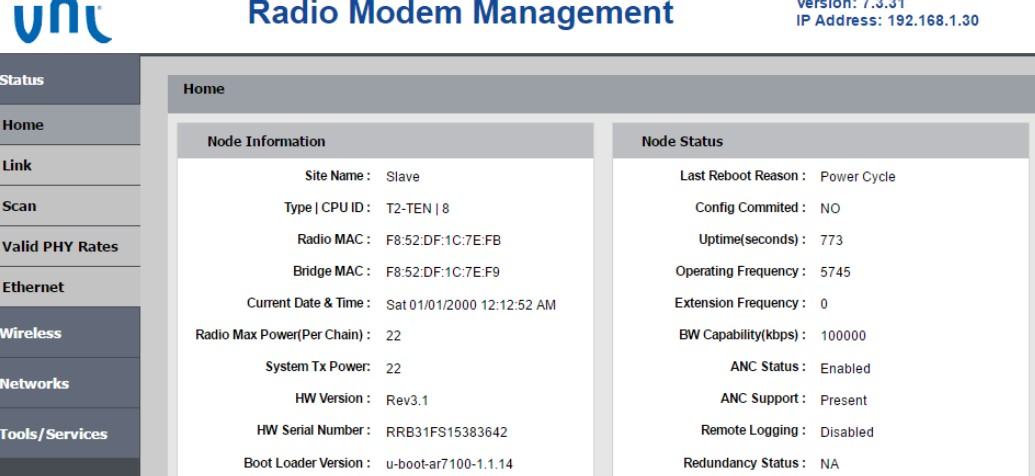
\includegraphics[width=0.5\textwidth]{img/vnl_rm.jpg}
		\caption{Pantalla principal \textit{Radio Modem Management}}
		\label{vnl_rm}
	\end{figure}

Por otra parte, la aplicación ofrece la posibilidad de configurar páginas de entrada por el usuario, permitiendo así una mayor personalización de la herramienta en función del perfil del usuario. Esta funcionalidad permite al usuario obtener datos en tiempo real del estado y actuación de los equipos involucrados en la red. 

\subsection{Equipos Mikrotik: NetMetal 5}
Los equipos NetMetal 5 son dispositivos pertenecientes a la familia de RouterBOARDS diseñadas y comercializadas por la empresa MikroTik \cite{Mikrotik}. Dicha empresa, se dedica al desarrollo de sistemas hardware y software inalámbricos en variedad de países a lo largo del mundo. El uso de sus equipos está extendido a nivel mundial debido a su bajo coste y a su alto rendimiento en sistemas de telecomunicaciones inalámbricas.
	\subsubsection{Hardware}
	Los equipos NetMetal disponen de un procesador MIPSBE que opera a 720MHzs y un recubrimiento hecho de aluminio y metal, su aspecto se muestra en la figura \ref{equipo}, lo que permite un gran rendimiento en zonas donde existen condiciones climatológicas adversas. El equipo está formado por tres puertos cuya funcionalidad es: la conexión de antenas externas en dos de ellos (permitiendo el uso de MIMO), y un terminal POE en el que se encuentran las entradas para la conexión mediante ethernet y la fuente de alimentación.
	\begin{figure}[H]
		\centering
		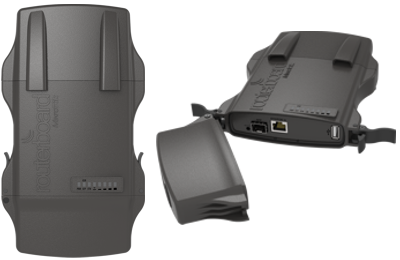
\includegraphics[width=0.5\textwidth]{img/netMetal5.png}
		\caption{Dispositivo NetMetal 5}
		\label{equipo}
	\end{figure}
	Existe una variante en los equipos, el cúal en vez de proporcionar tres entradas para antenas externas únicamente proporciona dos entradas.
	Los equipos NetMetal 5 son capaces de alcanzar altas tasas de transmisión en comunicaciones inalámbricas de larga distancia, gracias al uso del estándar 802.11ac y su eficiencia en cuánto al uso de los canales de 20/40/80 MHzs. Este hecho añadido a su robustez hacen de los equipos una elección idónea para el contexto del proyecto.\\
	Para llevar a cabo este Trabajo Fin de Grado, se han utilizados dos equipos NetMetal 5 como escenario de laboratorio.
	\subsubsection{Software}
	El sistema operativo que utilizan los equipos es RouterOS, propietario de MikroTik. Dicha distribución nos permite acceder al dispositivo de manera sencilla y configurar el equipo acorde al escenario requerido. Además de realizar configuraciones en cuánto a los parámetros deseados, el sistema operativo ofrece herramientas para la realización de pruebas a diferentes niveles de conectividad entre equipos. Los datos obtenidos, pueden ser procesados y representados de forma gráfica en tablas, diagramas y ficheros de texto. Independientemente de un formato u otro existe la posibilidad de exportar estos datos.\\\\
	
	Así mismo los equipos permiten exportar e importar las configuraciones realizadas siendo esto de gran utilidad a la hora de replicar una configuración en diferentes equipos. Por último este sistema operativo es compatible con cualquier distribución para PC, ofrece más de una variante para utilizar y configurar los equipos, ya sea mediante línea de comandos, interfaz web o utilizando la aplicación WinBox que se detalla a continuación.\\\\
	
	WinBox permite conectar los equipos de manera rápida y sencilla a través de su dirección IP o MAC, tal y como se muestra la siguiente figura \ref{inicioWinBox}. La configuración de usuario e IP vienen predeterminadas por el fabricante.\\
	Una vez logueado dentro del equipo, tal y como se muestra en la figura \ref{mainWinBox}, aparecen multitud de paneles y menús los cuáles nos servirán para configurar los equipos, ya sea en cuestiones de seguridad, creación de redes, configuración de interfaces, etc... Aparte de modificar la configuración que se establece predeterminada, WinBox ofrece la posibilidad de realizar mediciones para determinar el rendimiento de los equipos, como por ejemplo el número de paquetes envíado durante una transmisión.
		\begin{figure}[H]
			\centering
			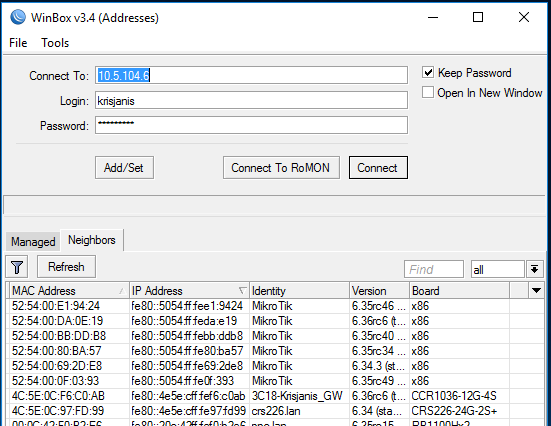
\includegraphics[width=0.7\textwidth]{img/winbox_loader.png}
			\caption{Pantalla loging en WinBox}
			\label{inicioWinBox}
		\end{figure}
		\begin{figure}[H]
			\centering
			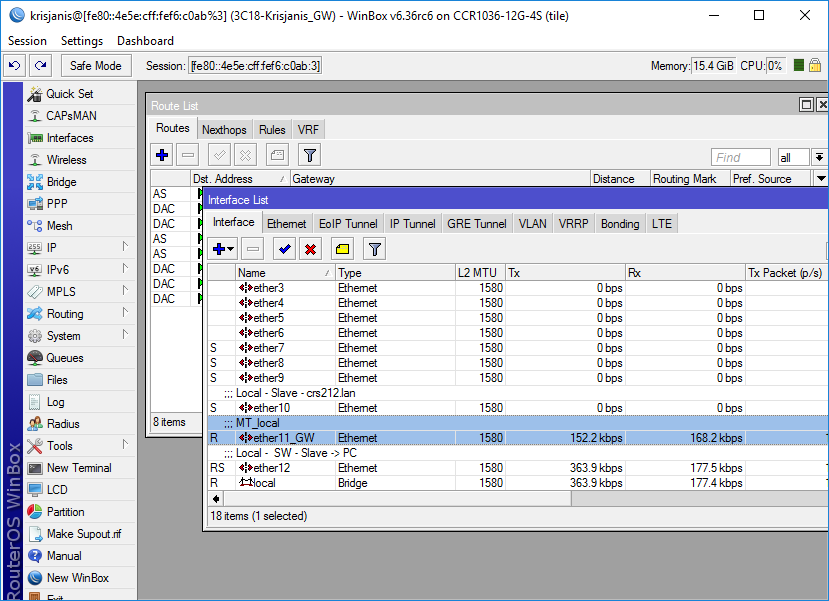
\includegraphics[width=0.7\textwidth]{img/winbox.png}
			\caption{Pantalla principal en WinBox}
			\label{mainWinBox}
		\end{figure}
		Al igual que la herramienta web, WinBox ofrece la posibilidad de utilizar una terminal compatible con el equipo y sistema operativo RouterOS. Dicha funcionalidad permite introducir y modificar las configuraciones existentes en los dispositivos, así cómo visualización de parámetros y realización de pruebas utilizando las herramientas integradas que posee el sistema operativo.
		
\section{Comparación entre equipos}	

		
\section{Configuración y diseño de la red}
Antes de realizar el montaje del escenario y realización de pruebas en laboratorio, debemos realizar un diseño y estudio sobre la red. Dicho análisis nos permitirá conocer de forma más detalla los diferentes factores que pueden comprometer la viabilidad de los diferentes enlaces que componen la red, y así ajustar la configuración de los equipos a dichos factores para garantizar el objetivo y requisitos predefinidos en el proyecto.\\\\

Tras la conlcusión de la parte correspondiente al estudio y diseño de la red, realizaremos nuestras simulaciones a nivel de laboratorio. El objetivo de esto, será establecer una comparación con los resultados obtenidos en la fase de estudio, para ello dispondremos de los equipos NetMetal 5 y ordenadores cuya distribución será Linux. Ya que los sistemas operativos pertenecientes a dicha distribución, otorgan facilidades a la hora de instalar y manejar los programas necesarios para la realización de pruebas. Las pruebas llevadas a cabo determinarán el rendimiento que ofrecen los equipos NetMetal 5 en lo que a conectividad y parámetros de calidad se refiere.

\subsection{Estudio previo} 
	En esta sección procederemos a realizar un estudio de forma cuantitativa con el objetivo de conocer cual sería el \textit{throughput} obtenido de forma teórica, por cada uno de los radioenlaces que forman la red del Napo. Para ello utilizaremos los valores empirícos obtenidos en el artículo \cite{simo2014assessing} recogidos en la tabla número 7,  pertenecientes al uso del protocolo NV2.\\\\
	
	Por una parte, los valores presentes en dicha tabla corresponden a medidas de capacidad en radioenlace para una distancia de 0 Km (medidas en laboratorio) y una distancia de 30 Km, las medidas fueron llevadas a cabo desde la modulación MCS0 hasta MCS15 para la mayoría de casos, salvo en las mediciones de 30 Km, qué para valores superiores a MCS11 no se pudieron realizar pruebas empirícas. No obstante, sólo nos apoyaremos y tomaremos como referencia los valores comprendidos entre la modulación MCS8 y MCS11 ya que son las modulaciones destinadas para el uso de MIMO. \\
	Por otra parte, dichas medidas corresponden a la utilización de 20 Mhz como ancho de banda, para poder establecer una relación con el ancho de banda utilizado en el proyecto se procederá a duplicar los valores obtenidos a 20 Mhz. Obteniendo así un aproximación de los valores teóricos que deberían ser obtenidos de forma empiríca para un ancho de banda de 40 Mhz; una vez concluida la parte teórica se contrastarán dichos valores con los obtenidos en laboratorio y se procederá a realizar un análisis más exhaustivo.\\\\
	
	Para poder llevar a cabo el estudio teórico, se han recogido los valores antes mencionados y se han organizado en pares de coordenadas obteniendo un conjunto de datos que establecen una relación entre: la distancia, \textit{throughput}, y el valor de la modulación MCS utilizado. Una vez acondicionados los datos se ha proyectado una recta lineal entre los puntos pertenecientes a cada MCS respecto a las coordenadas base de 0 Km y 30 Km, con el objetivo de obtener una recta que pase por todos los puntos de interés de nuestra red, tal y como muestra la figura \ref{rectaspendiente}, permitiendo establecer así una aproximación teórica de la capacidad del enlace en función de la distancia.\\\\
	
	De forma paralela, en base a la obtención de las rectas respecto a cada MCS hemos podido realizar una estimación de la capacidad teórica que debería de existir para cada radioenlace, dicha estimación se muestra en la figura \ref{valoresmbps}. Para llevar a cabo todo el estudio teórico y todo el desarrollo comentado anteriormente, se ha utilizado el script \ref{lst:script}, que está desarrollado en el lenguaje de programación Python, ya que permite la integración de módulos y librerías de análisis matemático de forma sencilla.
	
	\begin{figure}[H]
		\centering
		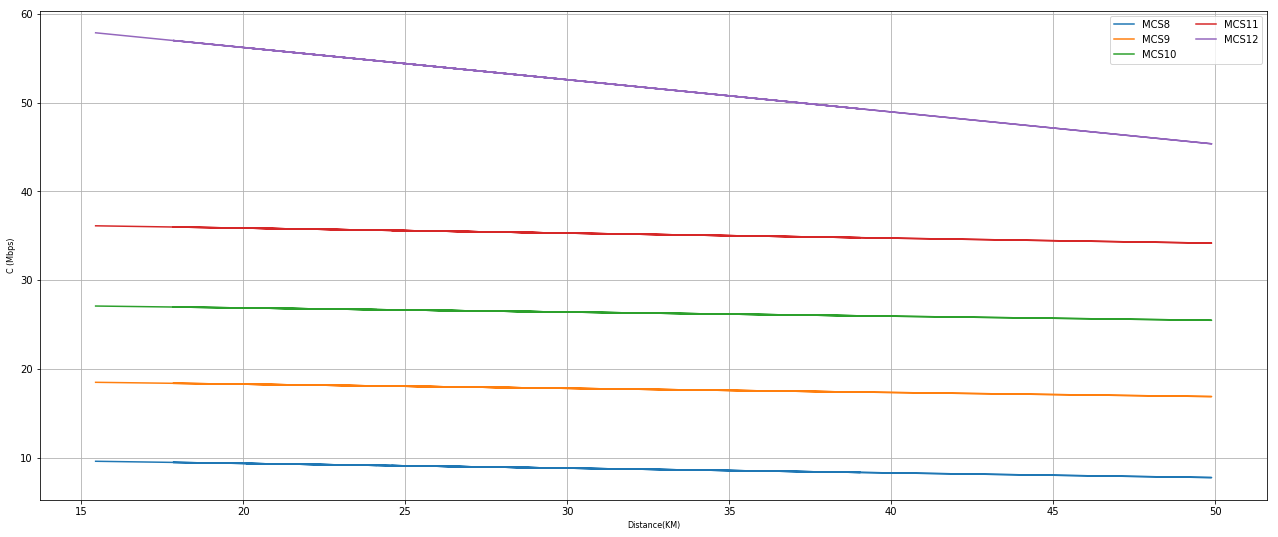
\includegraphics[width=0.7\textwidth]{img/rectas.png}
		\caption{Rectas lineales utilizando valores de 0 Km y 30 Km como coordenadas base}
		\label{rectaspendiente}
	\end{figure}
	
	\begin{figure}[H]
		\centering
		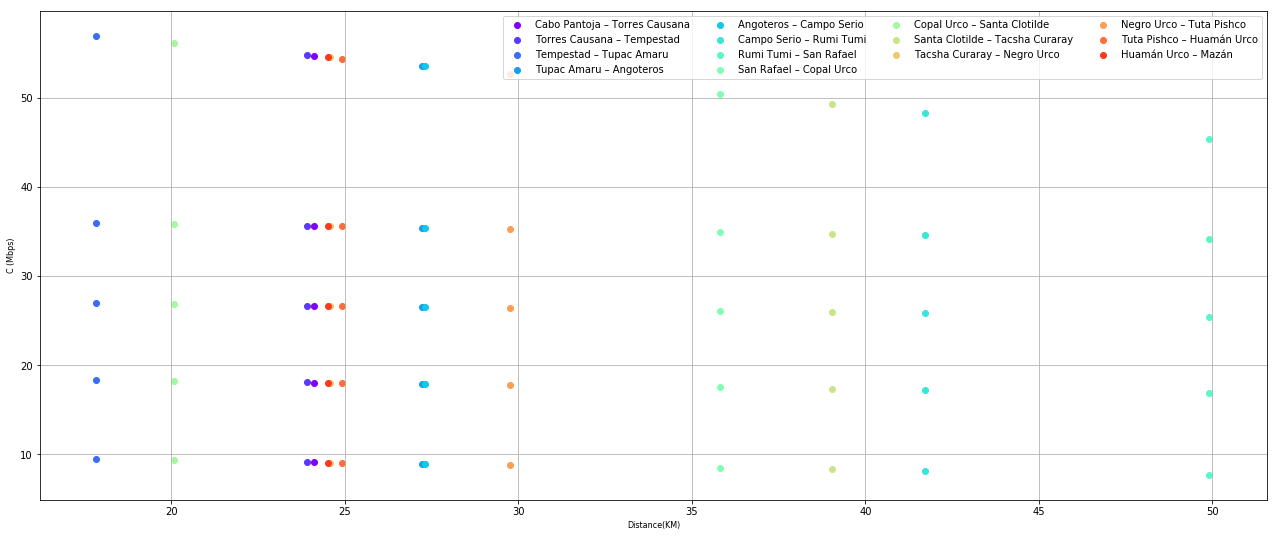
\includegraphics[width=0.7\textwidth]{img/valoresmbps.png}
		\caption{Capacidad del canal teórica respecto a la distancia para cada MCS con NV2}
		\label{valoresmbps}
	\end{figure}
	
	Los valores obtenidos y representados corresponden a las modulaciones comprendidas entre MCS8 y MCS12, no obstante el interés de este estudio es determinar cúal sería la modulación mínima utilizable de forma teórica en la red del Napo, asegurando así esa capacidad mínima definida de 44 Mbps por radioenlace. Cómo se ha comentado al inicio del capítulo se realizó una estimación para el ancho de banda correspondiente al proyecto, doblando los valores de \textit{throughput} existentes en las coordenadas base.\\\\
	
	En conclusión a este análisis teórico y aproximación analítica, la tabla \ref{table:capacidades} recoge los datos obtenidos, los cuáles reflejan que para cumplir con los requesitos necesarios de la red cada radioenlace debe utilizar una modulación MCS10.   
	
\subsection{Estudio con RadioMobile}
	Una vez desarrolado el estudio teórico sobre la red, nuestro siguiente paso será realizar una representación simulada con el objetivo de obtener más información sobre la viabilidad de enlace relativa a los emplazamientos del proyecto. Para ello, utilizaremos los datos de geolocalización y distancia relacionados con los emplazamientos de la red del Napo los cuáles se encuentran en las tablas \ref{table:distancias} y \ref{table:geolocalizacion}, para introducirlos en la herramienta RadioMobile y crear así nuestra red simulada. Junto a la localización geográfica y altura de cada emplazamiento tendremos que configurar los principales parámetros de la red y de los equipos en la herramienta, esta combinación nos permitirá obtener una aproximación sobre la calidad del enlace en términos generales e individuales de la red. A continuación se detallan las características de los sistemas insertados en la herramienta para llevar a cabo la simulación:
	\begin{itemize}
		\item Potencia de transmisión: 32 dBm
		\item Sensibilidad en recepción: -96 dBm
		\item Pérdidas por cable: 1,5 dB
		\item Ganancia de antena: 30 dBm
		\item Tipo de antena: Omnidireccional
		\item Frecuencia: 5260 MHzs
	\end{itemize}
	Una vez configurado los parámetros y características de los sistemas, obtenemos una representación simulada de la red tal y como se muestra en la figura \ref{redNapo}. Dicha simulación está sujeta al modelo \textit{Longley-Rice} que utiliza la variabilidad de tiempo, posición y situación para realizar los cálculos respecto al balance de enlace.  
	\begin{figure}[H]
		\centering
		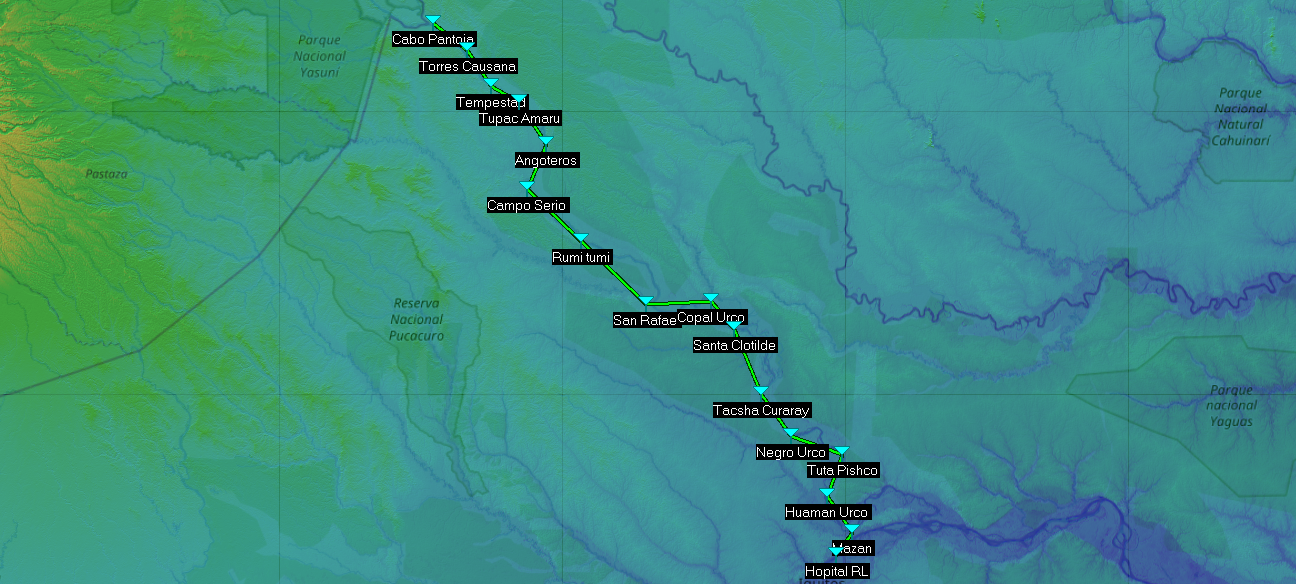
\includegraphics[width=0.7\textwidth]{img/redNapo.PNG}
		\caption{Representación de la red del Napo en RadioMobile}
		\label{redNapo}
	\end{figure}
	La funcionalidad \textit{Radio Link} que se encuentra dentro de RadioMobile, nos permite obtener una representación simulada del estado de cada radioenlace a través de la recreación del perfil geográfico y configuración de los sistemas involucrados en el enlace. Esto nos permite conocer los niveles de pérdidas, sensibilidad en recepción y margen dinámico de cada sistema de forma individual a través de la realización del balance de enlace. Dicho balance de enlace nos proporcionará información respecto a la sensibilidad y potencia en transmisión y recepción, para poder establecer la mínima tasa de transmisión soportada siempre y cuando, cumpla con los requisitos de viabilidad de enlace mencionados al principio de este Trabajo Fin de Grado.\\\\
	
	Para poder obtener una tasa mínima que cumpla los requisitos de transmisión mínimos mencionados en el capítulo de introducción, debemos tener en cuenta el tipo de tecnología que estamos utilizando. En nuestro caso, las transmisiones pertenencientes a la nueva red del Napo se realizarán utilizando la tecnología \textit{Multiple Input Multiple Output}, junto al uso de NV2 como protocolo de acceso al medio. La utilización de MIMO hace que nos centremos en los valores pertenecientes a las MCS cuyos valos están comprendidos entre MCS8 y MCS15, dichas MCS a su vez están formadas desde una constelación BPSK (formada por dos símbolos) hasta una 64-QAM (formada por 64 símbolos). Para poder establecer una comparación entre la modulación adecuada por cada radioenlace tendremos que comparar la senbilidad en recepción de cada sistema obtenido mediante la simulación, con los valores típicos de sensibilidad para dichas MCS.\\\\
	
	Los valores obtenidos a través de la simulación por cada radioenlace y los valores respecto al protocolo NV2 en términos de sensibilidad han sido recogidos en las siguientes tablas:\\\\
	
	En conclusión habiendo estudiado las diferentes situaciones y analizado las características de los radioenlaces cuyos resultados se recopilan en la siguiente tabla. En función de los valores obtenidos en la simulación y, teniendo en cuenta los resultados conseguidos mediante el estudio teórico previo, podemos destacar lo siguiente: 
	\begin{itemize}
		\item Existe línea de visión directa en la mayoría de casos, lo que implica asegurar la zona de Fresnel mínima para la viabilidad del enlace, en nuestro caso un sesenta por ciento.
		\item Habiendo analizado cada balance de enlace de forma individual podemos realizar una extrapolación para el total de la red, asegurando así un margen dinámico que garantice la viabilidad del enlace. En el caso del diseño inicial dicho margen dinámico era de 20 dB, por tanto habiendo contrastado los datos obtenidos con la simulación no existe compromiso respecto a la viabilidad de enlace en cada punto de la red.
		\item En base al estudio análitico hecho, para asegurar la total funcionalidad de la red, habría que utilizar un MCS10 como mínima para alcanzar una capacidad de enlace suficiente y necesaria.
	\end{itemize}
	
\subsection{Configuración de equipos}
Para poder recrear en laboratorio un escenario punto a punto de similares características a los de la red del Napo, utilizaremos dos equipos NetMetal 5 y dos portátiles con distribuciones Linux. Los ordenadores portátiles actuarán de emisor y receptor en nuestra red local junto a los equipos NetMetal 5 que interconectarán dichos terminales finales entre sí, como se muestra en la figura \ref{enlace}. Para obtener valores relacionados con los parámetros de QoS se inyectará tráfico con la herramienta Iperf y Bandwidth test, utilizando uno de los portátiles como cliente y otro como servidor.\\\\

\begin{figure}[H]
	\centering
	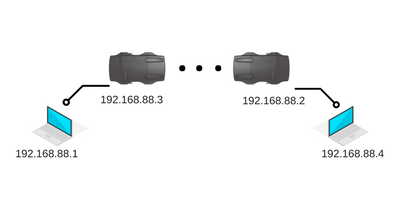
\includegraphics[width=0.7\textwidth]{img/escenario.png}
	\caption{Escenario de laboratorio punto a punto}
	\label{enlace}
\end{figure}

Antes de comenzar a detallar como se ha realizado la configuración a nivel de laboratorio de los equipos, debemos apuntar qué, en nuestro caso las antenas utilizadas son dipolos elementales colocados en posición vertical y horizontal transmitiendo forma multimodal, en el caso del proyecto Napo cada radioenlace constará de una antena parabólica colocada en lo alto de una infraestructura metálica, cuya ganancia de transmisión está en torno a los 30 dB. \\\\

\section{Inyección de tráfico simulado}
Para conocer el rendimiento y prestaciones de los equipos realizaremos pruebas a nivel de red a través de la inyección de tráfico simulado. Para llevar a cabo dicha prueba, utilizaremos el software disponible para los sistemas operativos de distribución Linux Iperf y la herramienta de medida de ancho de banda proporcionada por MikroTik Bandwidth text, las cuáles se detallan brevemente a continuación.\\\\

\subsection{Iperf}
Iperf \cite{Iperf} es una herramienta que permite realizar mediciones sobre el máximo rendimiento alcanzable respecto al ancho de banda y la calidad de un enlace red. Esto es posible mediante el análisis y recopilación de datos referentes a los protocolo de red TCP y UDP. Existe la variante Jperf, cuya única diferencia es la utilización de una interfaz gráfica en lugar de la entrada estándar de comandos.\\\\

La herramienta puede ser utilizada en modo cliente o en modo servidor, permitiendo realizar pruebas sobre la red hasta obtener los valores óptimos sobre la misma, tal y como se muestra en la figura \ref{logTestIperf}.\\
Esto es gracias al ajuste y modificación de parámetros que permite la herramienta: según sea nuestro escenario y el objetivo de nuestras pruebas, podremos obtener un tipo específico de datos u otros. La elección de los parámetros de la herramienta será diferente según el protocolo de red (TCP o UDP) que utilicemos en cada caso. A continuación detallamos las posibilidades que ofrece en base a cada uno de ellos:\\\\

En primer lugar explicaremos los parámetros relacionados al protocolo UDP, el cual nos permite seleccionar un ancho de bando específico en nuestra comunicación y permite utilizar multidifusión si fuera necesario. Además, los datos reportados por la herramienta en este caso son los relacionados con la pérdida de paquetes, ya sea en cuantía o en porcentaje, y las medidas relacionadas con el jitter y retardo.\\
En segundo lugar, los parámetros configurables respecto a TCP están relacionados con la elección de un tamaño de ventana TCP fijo para la comunicación, otorgando datos respecto al ancho de banda medido en la comunicación y el tamaño MSS/MTU.

\begin{figure}[H]
	\centering
	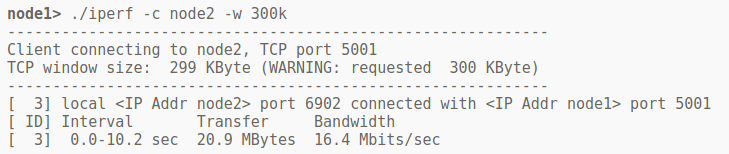
\includegraphics[width=0.7\textwidth]{img/log_iperf.png}
	\caption{Log obtenido al realizar una prueba con Iperf}
	\label{logTestIperf}
\end{figure}

\subsection{Bandwidth test}
\textit{Bandwidth test} es la herramienta desarrollada por el fabricante que nos permite realizar medidas entre equipos MikroTik en lo que a \textit{throughput} se refiere. Dicha herramienta está disponible tanto para la interfaz web, cómo para la consola.\\\\

Para llevar a cabo dicho test, debemos configurar uno de los routers que forman la red en modo servidor, y el resto en modo cliente, además la herramienta nos proporciona una serie de parámeotros configurables respecto a la red activa tales cómo: dirección, duración, tamaño de paquete, etc... \\
En función de estos parámetros el resultado de la prueba será de un modo u otro, y nos proporcionará los valores deseados respecto a el número de paquetes pérdidos, velocidades medias y totales en recepción y transmisión de la conexión activa. A continuación, en la figura \ref{logTest} se muestra un ejemplo del log obtenido al realizar una prueba utilizando la herramienta mencionada anteriormente.

\begin{figure}[H]
	\centering
	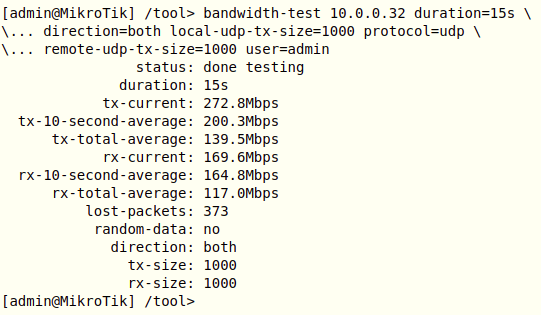
\includegraphics[width=0.7\textwidth]{img/log_test.png}
	\caption{Log obtenido al realizar una prueba sobre un enlace MikroTik activo}
	\label{logTest}
\end{figure}

\subsection{Configuración y realización de pruebas}

\section{Monitorización y gestión: Zabbix}
En esta sección se explicará la integración llevada a cabo con el escenario configurado en laboratorio y el \textit{software} de monitorización Zabbix. Así mismo, se procederá a explicar de manera más detallada el funcionamiento de la herramienta seleccionada en el marco contextual definido al inicio de este Trabajo Fin de Grado.\\\\

Antes de realizar la configuración del escenario formado en laboratorio, se procede a explicar cómo se va a llevar a cabo la integración de Zabbix y dicho escenario. Esto se llevará a cabo mediante el uso de plantillas XML y el protocolo SNMP el cúal, nos permite intercambiar información entre los dispositivos involucrados.\\
 
El protocolo SNMP (\textit{Simple Network Management Protocol}) es un protocolo que corresponde con la capa de aplicación y facilita el intercambio de información administrativa entre los dispositivos que componen una red, ya sean \textit{routers}, \textit{switches}, etc... Este protocolo facilita a los administradores de red conocer en todo momento el estado de la red, así cómo la posibilidad de interactuar con la misma tomando acciones de prevención, resolución de problemas y estudio sobre escalabilidad.\\
Para lograr esto, SNMP accede a la MIB (\textit{Management Information Base}) de los equipos. La MIB es una colección de información referente al equipo organizada de forma jerárquica mediante un árbol, para llevar a cabo una eficiente búsqueda y consulta de los objetos que se encuentran dentro del árbol, se organizan en subconjuntos denominados organizaciones.\\\\

Cada objeto, denominado OID (\textit{Object Identifier}) contiene un valor asociado al parámetro que representa, ya sea en formato de cadena de carácteres o en formato numérico, para conseguir dicho valor se ha de realizar una búsqueda descendente del árbol que forma la MIB, ya sea bien utilizando la nomenclatura numérica que tiene cada organización seguida de un punto (1.3.6....) o bien utilizando el nombre de cada organización seguido de un punto (iso.identified....). Ambos métodos permiten recuperar el valor del parámetro deseado y utilizarlo en nuestra integración.\\\\

Así mismo, el funcionamiento de SNMP involucra a los siguiente agentes:

\begin{itemize}
	\item Sistema administrador: Capaz de ejecutar aplicaciones (comandos) capaces de controlar los dispositivos involucrados en la red, proporcionando métricas útiles para el administrador en cuánto a los recursos del equipo.
	\item Dispositivo administrado: Equipo que contiene el agente SNMP y forma parte de la red recogiendo información usando el protocolo SNMP.
	\item Agente SNMP: Permite realizar una administración de la forma otorgada por el equipo de manera local y jerarquizarlo en forma de árbol y en un formato compatible al intercambio de información usando dicho protocolo.
\end{itemize}

SNMP no sólo nos permite recorrer el árbol MIB y obtener información de los equipos, sino que mediante aplicaciones (comandos), es posible realizar simples operaciones sobre la estructura jerarquizada de los equipos, dichos comando se describen a continuación:

\begin{itemize}
	\item Lectura/Escritura: Permiten al administrador leer/modificar los valores de las variables almacenados dentro de los dispositivos.
	\item Notificación: Permite a los equipos reportar eventos de manera asíncrona al administrador. 
	\item Transversales: Permiten a los equipos recolectar información de los elementos cercanos en la red y conformar tablas relacionadas a la información obtenida. 
\end{itemize}

\subsection{Integración de escenario}
Una vez explicado todo lo que implica el uso de SNMP y la jerarquización de los objetos existente en los equipos y cómo es posible realizar consultas a dichos objetos, procedemos a explicar cómo se va a integrar la información procedente de los equipos con Zabbix. Una de las facilidades que nos ofrece la herramienta es que podemos crear \textit{items} tal y como se muestra en la figura \ref{xmlTest}, aprovechando la información que nos proporcionan los OIDs en función de los parámetros que deseemos monitorizar. Para ello deberemos seguir el estándar XML, utilizando una plantilla como la mencionada antes e importarla en el sistema. De igual forma, que podemos importar datos existe la posibilidad de exportarlos, ofreciendo así versatilidad a la hora de integrar cualquier equipo en un sistema diferente. En el marco del proyecto los principales parámetros de interés son los referentes a salud de los equipos (carga CPU, temperatura, etc...) y a tráfico obtenido. 

\begin{figure}[H]
	\centering
	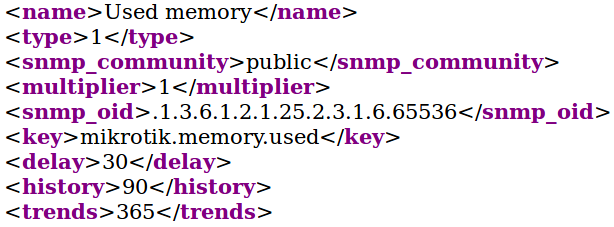
\includegraphics[width=0.7\textwidth]{img/xml_example.png}
	\caption{Ejemplo de configuración de un item sobre XML en Zabbix}
	\label{xmlTest}
\end{figure}

Una vez cargados los dispositivos involucrados en la plataforma, Zabbix ofrece varias herramientas para realizar un seguimiento sobre dichos elementos y otorgar control total sobre ellos al administrador, como por ejemplo configurando \textit{dashboards} de seguimiento, alertas sobre equipos, creación de mapas de redes, etc... A continuación se procede a detallar algunas de las aplicaciones utilizadas en este Trabajo Fin de Grado cuyo objetivo es monitorizar y obtener un control total de la red:\\\\

En primer lugar, nos hemos centrado en la representación gráfica del rendimiento que otorgan los equipos a nivel de red, para ello, hemos utilizado la aplicación que ofrece la propia herramienta que permite realizar gráficas a nivel de interfaz, como se muestra en la figura \ref{zabbixMeasure}, una aplicación interesante de estas gráficas es que se puede realizar un tablero configurable conjunto, es decir, integrar dicha gráfica (o similares) de diferentes dispositivos en un único tablero, otorgando así al administrador una visión global del tráfico entrante y saliente de la red en conjunto.

\begin{figure}[H]
	\centering
	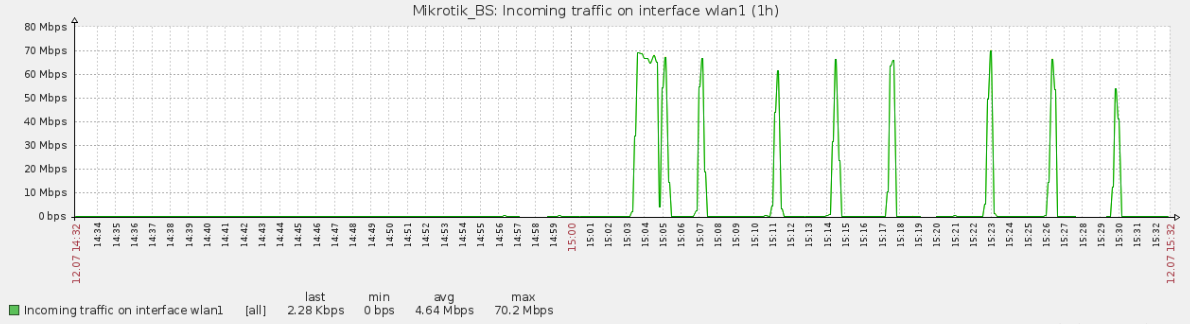
\includegraphics[width=0.7\textwidth]{img/zabbix_measure.png}
	\caption{Ejemplo de representación gráfica de tráfico mostrado en un Dashboard de Zabbix}
	\label{zabbixMeasure}
\end{figure}

En segundo lugar, Zabbix ofrece alertas configurables en función de los \textit{items} cargados en la plantilla XML tal y como se muetra en la figura , esto quiere decir que la herramienta ofrece \textit{triggers} configurables, ya sea bien de forma predeterminada o personalizada, que permiten establecer valores umbral para los diferentes niveles de alerta que ofrece la herramienta, generando así una categorización de problemas y otorgando al administrador una versión prioritaria de la acción que ha de ser tomada. Las alertas no son configuradas únicamente si el programa se está ejecutando en primer plano, Zabbix ofrece una extensión llamada PostFix \cite{PostFix} que permite integrar y configurar alertas para que sean enviadas mediante email.\\
De igual forma, Zabbix mantiene un archivo histórico de logs el cúal otorga cierta ventaja a la hora de actuar al administrador, ya sea en labores de mantemiento de la red o bien en labores predictivas. 

\begin{figure}[H]
	\centering
	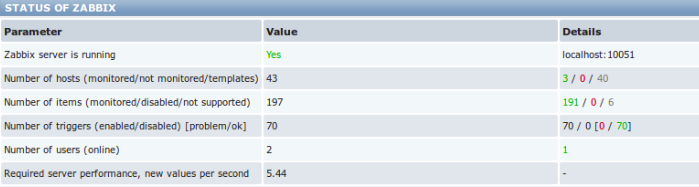
\includegraphics[width=0.7\textwidth]{img/zabbix_resume.png}
	\caption{Ejemplo del estado de la red en Zabbix}
	\label{zabbixResume}
\end{figure}

Por último, otra aplicación interesante en el marco del proyecto es la creación de mapas de red, como muestra la figura \ref{zabbixNetwork}, la cúal permite al administrador no sólo jerarquizar los equipos en función de nombres o por IPs, si no que otorga la posibilidad de subdividir una red total en subredes de forma que puedan aislarse cada una de ellas en subconjuntos, consiguiendo así un análisis más rápido y eficaz que si tuviera que realizarse de toda la red en conjunto. Aparte de esto, subdividir las redes porporciona la capacidad de asignar cada subred a un grupo de técnicos determinado evitando así que la gestión de una única subred involucre al resto de la misma.

\begin{figure}[H]
	\centering
	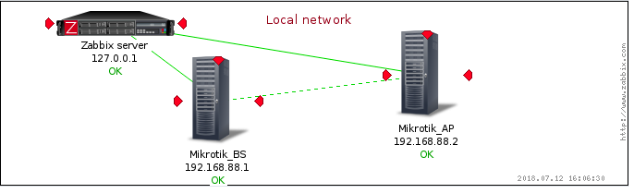
\includegraphics[width=0.7\textwidth]{img/zabbix_networks.png}
	\caption{Ejemplo de jerarquización de redes en Zabbix}
	\label{zabbixNetwork}
\end{figure}

En definitiva y reuniendo todo lo explicado a lo largo de este capítulo, Zabbix no sólo es una solución que cumple con los requisitos mínimos de monitorización de redes requeridos en el proyecto, si no que su amplia variedad de integraciones y aplicaciones.Zabbix no sólo permite una fácil integración con los dispositivos físicos mediante el uso de plantilla XML y protocolo SNMP, si no que también ofrece una solución a todo lo referido con \textit{software} de terceros. Todo esto a partir de la editabilidad de la mayor parte su funcionalidad básica para hacer que el administrador de redes tenga la mayor cantidad de información sobre los equipos, concentrada de tal forma que su actuación se inminente y precisa si esta fuera requerida.